\documentclass[11pt]{article}
\usepackage[margin=1in]{geometry}
\usepackage{amsmath,amssymb,amsthm,mathtools}
\usepackage{booktabs}
\usepackage{graphicx}
\usepackage{tikz}
\usetikzlibrary{arrows.meta,positioning,backgrounds}
\usepackage{hyperref}
\usepackage{longtable}
\usepackage{array}
\newtheorem{theorem}{Theorem}
\newtheorem{lemma}[theorem]{Lemma}
\newtheorem{proposition}[theorem]{Proposition}
\newtheorem{corollary}[theorem]{Corollary}
\newtheorem{definition}[theorem]{Definition}
\newtheorem{remark}[theorem]{Remark}
\newenvironment{sourceresult}[1]{\par\medskip\noindent\textbf{#1.}\ \itshape}{\par\medskip}
\sloppy
\emergencystretch=3em

\title{Formal Verification Report: powers\_of\_two\_reach\_one\\[0.5em]{\large Source: Self-authored demonstration problem, this session, no external publication}}
\author{Black Swan Labs FCVE \\ ledger through EVENT-012}
\date{2026-09-19}
\begin{document}
\maketitle

\noindent\textbf{Trust Statement.} The formal result was checked using Lean 4.34.0 under the pinned project environment (Mathlib master 5ed2965). The theorem CLAIM-002 was kernel-checked with axiom footprint propext, Quot.sound. Independent checking status is INDEPENDENTLY\_CHECKED (recorded before the Section 17 vocabulary existed, as PASS). Computational/adversarial testing produced: COMPUTATIONALLY\_SUPPORTED; NO\_COUNTEREXAMPLE\_FOUND\_IN\_TESTED\_DOMAIN (diagnostic only). The remaining trust limitations are: The report (Gate 12) was not recorded; The repository, commit and toolchain were captured after the run (on 2026-09-19), not recorded during it; they describe the project as it is now; The checker used for the independent check is not identified in the record; only its result is; The Gate 8 search examined only k = 0 to 20 and k = 50, 100, 500, 1000. This report does not claim that computational testing constitutes formal proof or that formalization alone establishes the truth of the original informal statement.

\begin{abstract}
This report documents the formal verification of powers\_of\_two\_reach\_one (CLAIM-002) under the Formal Claim Verification Engine. Recorded: build PASS -- 8924/8924 jobs, exit 0, no sorry/admit; axiom footprint propext, Quot.sound; independent check INDEPENDENTLY\_CHECKED (recorded before the Section 17 vocabulary existed, as PASS). Computational testing is diagnostic and is not proof. Section 17 states the status the recorded evidence permits; the governance decision is recorded separately, after this report.
\end{abstract}

\section{Mathematical Statement}
\begin{sourceresult}{powers\_of\_two\_reach\_one}
Every power of two reaches 1 under the standard Collatz function: for f(n) = n/2 if n even, 3n+1 if n odd, and for every k >= 0, iterating f starting from 2\textasciicircum{}k eventually reaches 1.
\end{sourceresult}
Source: Self-authored demonstration problem, this session, no external publication. Source location: source/original.md.

\section{Definitions and Assumptions}
\subsection*{Definitions}
\begin{itemize}
\item f: N -> N (called collatzStep in the Lean formalization), f(n) = n/2 if n even, 3n+1 if n odd -- this is the STANDARD (uncompressed) Collatz map, distinct from Eliahou's compressed map T used in VCE-001
\end{itemize}
\subsection*{Source assumptions}
\begin{itemize}
\item \textbf{SA-001} k is a natural number, k >= 0
\end{itemize}
\subsection*{Formalization assumptions}
\begin{itemize}
\item \textbf{FA-001} 'iterating f m times' is represented via Mathlib's Function.iterate (f\textasciicircum{}[m]), a standard, well-understood construction with no hidden semantics beyond repeated function application
\end{itemize}
\subsection*{Computational assumptions}
None recorded.
\section{Proof Outline}
\begin{enumerate}
\item \textbf{method.} induction on k
\item \textbf{base case.} k=0: 2\textasciicircum{}0=1, already at 1 in 0 steps
\item \textbf{inductive step.} 2\textasciicircum{}(k+1) is even, one step of f sends it to 2\textasciicircum{}k; by induction hypothesis 2\textasciicircum{}k reaches 1 in m more steps, so 2\textasciicircum{}(k+1) reaches 1 in m+1 steps
\end{enumerate}
\section{Proof Dependency Diagram}
\begin{center}
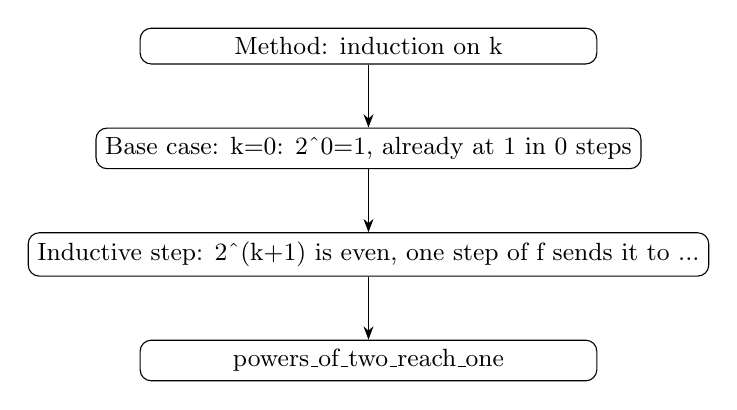
\begin{tikzpicture}[box/.style={draw,rounded corners,align=center,minimum width=58mm,font=\small}, node distance=8mm, >=Stealth]
\node[box] (s0) {Method: induction on k};
\node[box, below=of s0] (s1) {Base case: k=0: 2\textasciicircum{}0=1, already at 1 in 0 steps};
\draw[->] (s0) -- (s1);
\node[box, below=of s1] (s2) {Inductive step: 2\textasciicircum{}(k+1) is even, one step of f sends it to ...};
\draw[->] (s1) -- (s2);
\node[box, below=of s2] (goal) {powers\_of\_two\_reach\_one};
\draw[->] (s2) -- (goal);
\end{tikzpicture}
\end{center}
\section{Formalization}
Lean identifiers below are cross-references; the mathematics is in the sections above (\S{}29).
\subsection*{powers\_of\_two\_reach\_one}
{\footnotesize\ttfamily\raggedright\hangindent=1.4em\hangafter=1\noindent
\hspace*{0.00em}theorem powers\_\allowbreak{}of\_\allowbreak{}two\_\allowbreak{}reach\_\allowbreak{}one : \ensuremath{\forall} k : \ensuremath{\mathbb{N}}, \ensuremath{\exists} m : \ensuremath{\mathbb{N}}, (collatzStep\textasciicircum{}[m]) (2 \textasciicircum{} k) = 1\par
}

\section{Semantic Bridge}
\subsection*{Informal Statement}
Every power of two reaches 1 under the standard Collatz function: for f(n) = n/2 if n even, 3n+1 if n odd, and for every k >= 0, iterating f starting from 2\textasciicircum{}k eventually reaches 1.
\subsection*{Normalized Statement}
\subsection*{Normalized Claim: CLAIM-002}
\subsubsection*{Objects and domains}
\begin{itemize}
\item $f : \mathbb{N} \to \mathbb{N}$, $f(n) = \begin{cases} n/2 & n \text{ even} \\ 3n+1 & n \text{ odd} \end{cases}$ --- the \textbf{standard} (uncompressed) Collatz map. (Note: this is a different map from Eliahou's compressed $T$ used in VCE-001, which folds the forced halving after an odd step into one combined step. $f$ and $T$ are related but not identical.)
\item $f^{(m)}$ denotes $f$ composed with itself $m$ times.
\end{itemize}
\subsubsection*{The claim}
\textbf{Given}: $k \in \mathbb{N}$.

\textbf{Conclusion}: $\exists\, m \in \mathbb{N}$ such that $f^{(m)}(2^k) = 1$.

\subsubsection*{Why this is true}
By induction on $k$.

\begin{itemize}
\item \textbf{Base case} ($k=0$): $2^0 = 1$, so $m=0$ works trivially.
\item \textbf{Inductive step}: assume $f^{(m)}(2^k) = 1$ for some $m$. Since $2^{k+1}$ is even, $f(2^{k+1}) = 2^{k+1}/2 = 2^k$. So $f^{(m+1)}(2^{k+1}) = f^{(m)}(f(2^{k+1})) = f^{(m)}(2^k) = 1$.
\end{itemize}
This is a completely elementary, fully constructive argument --- no case analysis beyond parity, no external results needed.

\subsubsection*{Status}
\textbf{MATCH} --- direct restatement, nothing to disambiguate.


\subsection*{Lean Statement}
{\footnotesize\ttfamily\raggedright\hangindent=1.4em\hangafter=1\noindent
\hspace*{0.00em}theorem powers\_\allowbreak{}of\_\allowbreak{}two\_\allowbreak{}reach\_\allowbreak{}one : \ensuremath{\forall} k : \ensuremath{\mathbb{N}}, \ensuremath{\exists} m : \ensuremath{\mathbb{N}}, (collatzStep\textasciicircum{}[m]) (2 \textasciicircum{} k) = 1\par
}

\subsection*{Differences}
\subsection*{Gate 4: Lean Formalization Comparison --- CLAIM-002}
\begin{center}\small\begin{tabular}{p{0.46\textwidth}p{0.46\textwidth}}\toprule
Human mathematics (normalized) & Lean \\ \midrule
$f(n) = n/2$ if even, $3n+1$ if odd & \texttt{def collatzStep (n : \ensuremath{\mathbb{N}}) : \ensuremath{\mathbb{N}} := if n \% 2 = 0 then n / 2 else 3 * n + 1} \\
$\forall k,\ \exists m,\ f^{(m)}(2^k)=1$ & \texttt{theorem powers\_of\_two\_reach\_one : \ensuremath{\forall} k : \ensuremath{\mathbb{N}}, \ensuremath{\exists} m : \ensuremath{\mathbb{N}}, (collatzStep\textasciicircum{}[m]) (2 \textasciicircum{} k) = 1} \\
Induction on $k$, base case $2^0=1$, step: $2^{k+1}\to 2^k$ via one even step & \texttt{induction k with | zero => exact \ensuremath{\langle}0, rfl\ensuremath{\rangle} | succ n ih => ...} --- identical structure \\
\bottomrule\end{tabular}\end{center}
\subsubsection*{Checklist}
\begin{center}\small\begin{tabular}{p{0.46\textwidth}p{0.46\textwidth}}\toprule
Check & Finding \\ \midrule
Stronger/weaker & Neither --- exact match \\
Altered domain & No \\
Missing/extra hypothesis & None \\
Changed quantifier & No \\
Changed function & No --- \texttt{collatzStep} is exactly $f$ as normalized \\
Coercion & None needed (pure \ensuremath{\mathbb{N}} arithmetic throughout) \\
Finite/infinite mismatch & No \\
\bottomrule\end{tabular}\end{center}
This is the simplest possible Gate 4 outcome: the Lean statement is a direct

transliteration of the normalized claim, and the proof's induction structure

matches the normalized proof step-for-step (base case \texttt{k=0}, inductive step

using \texttt{Function.iterate\_succ} to peel off exactly one application of

\texttt{collatzStep}, matching the normalized argument's "$f(2^{k+1})=2^k$, then

apply the inductive hypothesis").

\subsubsection*{Status: MATCH}

\subsection*{Findings recorded by the reviewer}
No difference was found by any of the required checks; each check records its basis in the semantic record.
\subsection*{Justification}
Gate 4 records the Lean statement as a direct transliteration of the normalized claim (same function, domain, quantifiers, conclusion) and the proof's induction structure matches the normalized argument step for step. The Gate 7 re-audit found no undisclosed change, and the axiom footprint contains no classical assumption.


\subsection*{Verdict}
\noindent\textbf{FAITHFUL}\par Set by Wilson. Recorded context: Gate 4 recorded MATCH; Gate 7 recorded PASS -- no undisclosed semantic change; axiom footprint itself serves as independent corroboration of the re-audit's conclusion.
\section{Lean Environment}
\begin{tabular}{@{}ll@{}}
\toprule
Lean Version & 4.34.0 \\
Mathlib Version & master 5ed2965 \\
\bottomrule
\end{tabular}
\section{Formal Verification}
PASS -- 8924/8924 jobs, exit 0, no sorry/admit.
Source of this field: ledger:EVENT-006.
\section{Axiom Audit}
Actual axiom footprint: propext, Quot.sound.
Source: parsed-legacy-text:EVENT-007.
\section{Independent Check}
PASS -- Checked 1662 declarations with no errors. Axioms confirmed: propext, Quot.sound (matches Gate 6 exactly).  (legacy wording).
Recording the checker and its version does not by itself establish independence (\S{}17).
\section{Computational / Adversarial Tests}
Counterexample search: COMPUTATIONALLY\_SUPPORTED -- all cases reach 1 in exactly k steps as predicted; no counterexample in tested domain [diagnostic, not proof]

Computational test: NO\_COUNTEREXAMPLE\_FOUND\_IN\_TESTED\_DOMAIN -- 5001 cases over: every integer k in [0,5000]; full trajectory 2\textasciicircum{}k..1; two independent implementations of f; NOT PROOF [diagnostic, not proof]

Neither result is formal proof (\S{}16, \S{}18).
\subsection*{What these tests do not establish}
\begin{itemize}
\item They are not proof of the claim (Sections 16 and 18). A search that finds no counterexample is diagnostic evidence only.
\item The tested domain is not recorded for these results, so this report cannot say which cases were examined.
\item The Gate 8 search examined k = 0 to 20 and k = 50, 100, 500 and 1000 only; no other values of k were tested by that script. (stated by Wilson)
\end{itemize}
\section{Verification Limitations}
\begin{longtable}{p{0.16\textwidth}p{0.78\textwidth}}
\toprule Item & Limitation \\ \midrule \endhead
1 & The report (Gate 12) was not recorded. \\
2 & The repository, commit and toolchain were captured after the run (on 2026-09-19), not recorded during it; they describe the project as it is now. \\
3 & The checker used for the independent check is not identified in the record; only its result is. \\
4 & The Gate 8 search examined k = 0 to 20 and k = 50, 100, 500 and 1000 only; no other values of k were tested by that script (stated by Wilson). \\
\midrule \multicolumn{2}{l}{\textit{Record-keeping notes (these do not change what the verification shows)}} \\ \midrule
5 & 10 of 12 ledger events predate the input/output hash fields and carry none. \\
6 & Events EVENT-009 (COMPUTATIONALLY\_SUPPORTED) used wording outside the Section 16 vocabulary; each is read as diagnostic evidence, not proof. \\
\bottomrule
\end{longtable}
\section{Verification Matrix}
\begin{longtable}{lllll}
\toprule Gate & Ledger action & Event & Status & Satisfied \\ \midrule \endhead
G0 & source intake & EVENT-001 & PASS & yes \\
G1 & claim extraction & EVENT-002 & PASS & yes \\
G2 & assumption extraction & EVENT-003 & PASS & yes \\
G3 & semantic normalization & EVENT-004 & PASS & yes \\
G4 & lean formalization comparison & EVENT-005 & PASS & yes \\
G5 & lean build & EVENT-006 & PASS & yes \\
G6 & axiom audit & EVENT-007 & PASS & yes \\
G7 & semantic re audit & EVENT-008 & PASS & yes \\
G8 & adversarial computational test & EVENT-009 & DIAGNOSTIC & yes \\
G9 & independent check & EVENT-010 & PASS & yes \\
G10 & computational check & EVENT-011 & DIAGNOSTIC & yes \\
G11 & evidence graph & EVENT-012 & PASS & yes \\
G12 & report generation & - & MISSING & no \\
ORDER & canonical chain (\S{}2) & - & PASS & yes \\
\bottomrule
\end{longtable}
\section{Trust / Verification Chain}
\begin{center}
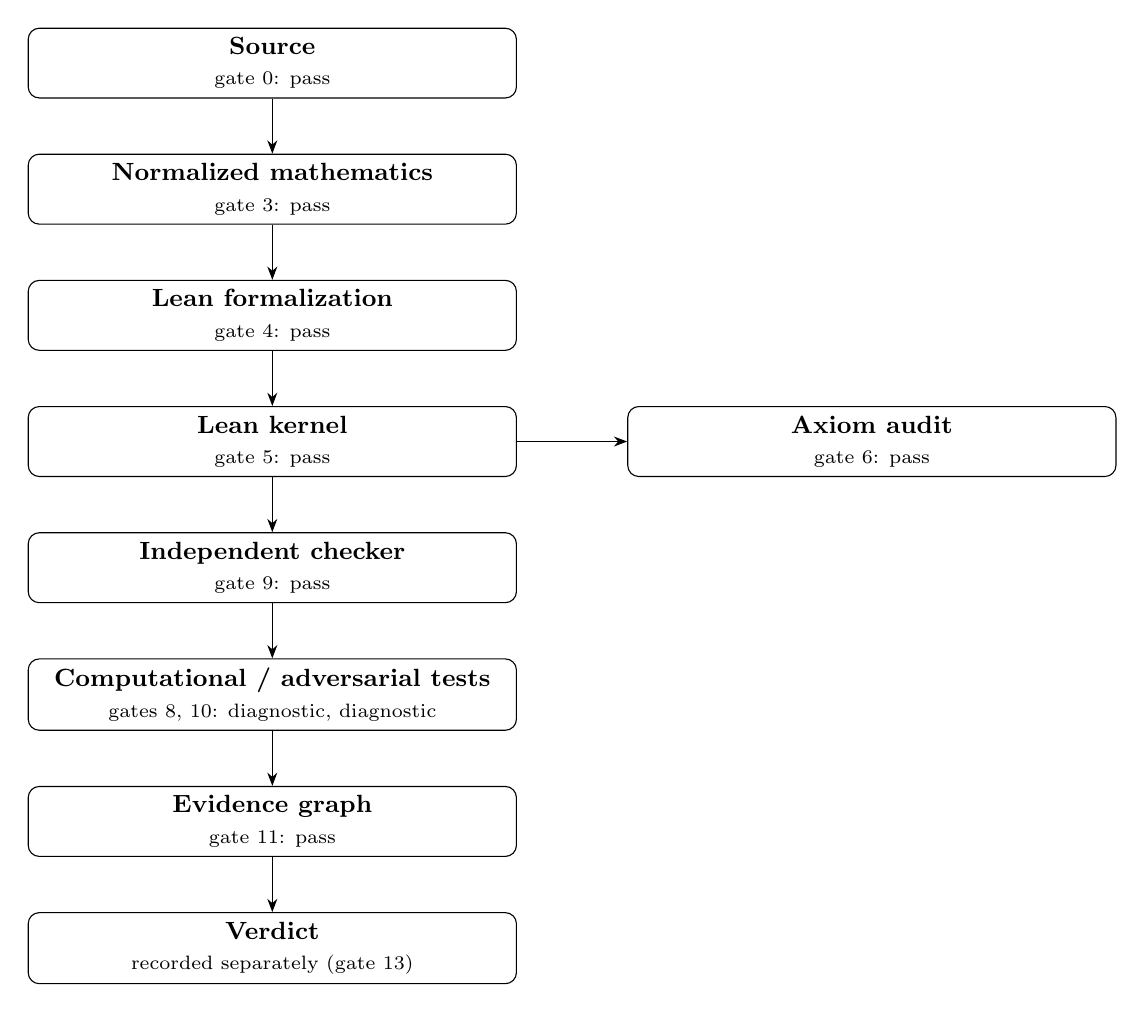
\begin{tikzpicture}[node distance=7mm, box/.style={draw,rounded corners,align=center,minimum width=62mm,font=\small}, >=Stealth]
\node[box] (src) {\textbf{Source}\\{\scriptsize gate 0: pass}};
\node[box, below=of src] (norm) {\textbf{Normalized mathematics}\\{\scriptsize gate 3: pass}};
\draw[->] (src) -- (norm);
\node[box, below=of norm] (lean) {\textbf{Lean formalization}\\{\scriptsize gate 4: pass}};
\draw[->] (norm) -- (lean);
\node[box, below=of lean] (kern) {\textbf{Lean kernel}\\{\scriptsize gate 5: pass}};
\draw[->] (lean) -- (kern);
\node[box, below=of kern] (chk) {\textbf{Independent checker}\\{\scriptsize gate 9: pass}};
\draw[->] (kern) -- (chk);
\node[box, below=of chk] (comp) {\textbf{Computational / adversarial tests}\\{\scriptsize gates 8, 10: diagnostic, diagnostic}};
\draw[->] (chk) -- (comp);
\node[box, below=of comp] (evd) {\textbf{Evidence graph}\\{\scriptsize gate 11: pass}};
\draw[->] (comp) -- (evd);
\node[box, below=of evd] (ver) {\textbf{Verdict}\\{\scriptsize recorded separately (gate 13)}};
\draw[->] (evd) -- (ver);
\node[box, right=14mm of kern] (ax) {\textbf{Axiom audit}\\{\scriptsize gate 6: pass}};
\draw[->] (kern) -- (ax);
\end{tikzpicture}
\end{center}
\section{Reproducibility Instructions}
\begin{tabular}{@{}p{0.27\textwidth}p{0.68\textwidth}@{}}
\toprule
Repository URL & NOT RECORDED \\
Commit & 409c4c3b6f0179\allowbreak{}ae9131ac245099\allowbreak{}8e59a7fb1132 (working tree clean) \\
Project directory (now) & /Users/lordwil\allowbreak{}son/ico-collat\allowbreak{}z/ico\_collatz\_\allowbreak{}verification \\
Lean toolchain file & leanprover/lea\allowbreak{}n4:v4.34.0 \\
Lean version & 4.34.0 \\
Lake version & Lake version 5.0.0-src+293d\allowbreak{}5d0 (Lean version 4.34.0) \\
Mathlib revision & master 5ed2965 (commit 5ed2965256430c\allowbreak{}3649e86755f957\allowbreak{}6b54eca72435) \\
Checker & NOT RECORDED \\
Expected build result & PASS -- 8924/8924 jobs, exit 0, no sorry/admit \\
How these were obtained & Captured 2026-09-19 from the project as it is now; not recorded during the run \\
Matches the commit the run's notes name & not checked \\
\bottomrule
\end{tabular}

{\footnotesize\ttfamily\raggedright\hangindent=1.4em\hangafter=1\noindent
\hspace*{0.00em}\# repository location and commit were not recorded for this run (see table above)\par
\hspace*{0.00em}cat lean-toolchain\par
\hspace*{0.00em}lake --version\par
\hspace*{0.00em}lean --version\par
\hspace*{0.00em}lake build IcoCollatzVerification.\allowbreak{}PowersOfTwoReachOne\par
\hspace*{0.00em}\# in a Lean file importing the module:  \#print axioms powers\_\allowbreak{}of\_\allowbreak{}two\_\allowbreak{}reach\_\allowbreak{}one\par
\hspace*{0.00em}\# independent-check commands were not recorded for this run\par
}

The repository facts were captured after the run and describe the project as it is now; they do not prove what the original run built. The build command is the one recorded in EVENT-006.
Reproducibility level supported by recorded evidence: R4. This tool did not re-run the build.
\section{Correction Ledger}
No failed or disputed gate results are recorded in the ledger.


\section{Conclusion}
The recorded evidence is summarized in the Trust Statement and the verification matrix above. Recorded failure is not a passed gate.
\begin{center}\begin{tabular}{@{}p{0.36\textwidth}p{0.58\textwidth}@{}}
FORMAL PROOF (build): & PASS \\
AXIOM AUDIT: & PASS \\
SEMANTIC MATCH (Gate 4): & PASS \\
SEMANTIC RE-AUDIT (Gate 7): & PASS \\
INDEPENDENT CHECK: & PASS \\
COUNTEREXAMPLE SEARCH: & NO COUNTEREXAMPLE FOUND IN TESTED DOMAIN (diagnostic, not proof) \\
COMPUTATIONAL TEST: & NO COUNTEREXAMPLE FOUND IN TESTED DOMAIN (diagnostic, not proof) \\
REPRODUCIBILITY: & R4 (ceiling supported by recorded evidence) \\
\end{tabular}\end{center}
%% PERMITTED-STATUS-BEGIN
\begin{quote}\textbf{Status the evidence permits.} The recorded evidence satisfies the conditions for promotion (Section 53), assuming this report itself compiles cleanly, which is recorded afterwards as Gate 12. Whether to promote is the reviewer's decision, recorded after this report. This is not a decision: the governance decision is recorded as a separate step after this report.\end{quote}
%% PERMITTED-STATUS-END
\appendix
\section{Lean Source}
{\footnotesize\ttfamily\raggedright\hangindent=1.4em\hangafter=1\noindent
\hspace*{0.00em}theorem powers\_\allowbreak{}of\_\allowbreak{}two\_\allowbreak{}reach\_\allowbreak{}one : \ensuremath{\forall} k : \ensuremath{\mathbb{N}}, \ensuremath{\exists} m : \ensuremath{\mathbb{N}}, (collatzStep\textasciicircum{}[m]) (2 \textasciicircum{} k) = 1\par
}

\section{Tests}
\begin{itemize}
\item \textbf{EVENT-009} python3 verification-002/computational/tests/verify\_powers\_of\_two.py: COMPUTATIONALLY\_SUPPORTED -- all cases reach 1 in exactly k steps as predicted; no counterexample in tested domain
\item \textbf{EVENT-011} python Python 3.12.9: verify\_gate10.py: NO\_COUNTEREXAMPLE\_FOUND\_IN\_TESTED\_DOMAIN -- 5001 cases over: every integer k in [0,5000]; full trajectory 2\textasciicircum{}k..1; two independent implementations of f; NOT PROOF
\end{itemize}
\section{Evidence Receipt}
\begin{longtable}{p{0.24\textwidth}p{0.70\textwidth}}
\toprule Field & Value \\ \midrule \endhead
SOURCE HASH & sha256:97d49fb\allowbreak{}c3576e79f3901c\allowbreak{}e85f0fb9dd92d9\allowbreak{}cbf06d6beb933a\allowbreak{}ada6a2f1a194d6\allowbreak{}0 (../verificati\allowbreak{}on-002/source/\allowbreak{}original.md) \\
THEOREM ID & CLAIM-002 (powers\_of\_two\allowbreak{}\_reach\_one) \\
CLAIM & Every power of two reaches 1 under the standard Collatz function: for f(n) = n/2 if n even, 3n+1 if n odd, and for every k >= 0, iterating f starting from 2\textasciicircum{}k eventually reaches 1. \\
NORMALIZED CLAIM & verification-0\allowbreak{}02/normalized/\allowbreak{}normalized-cla\allowbreak{}im.md -- MATCH \\
LEAN STATEMENT & Gate 4: MATCH \\
LEAN VERSION & 4.34.0 \\
MATHLIB VERSION & master 5ed2965 \\
BUILD RESULT & PASS -- 8924/8924 jobs, exit 0, no sorry/admit \\
AXIOM FOOTPRINT & propext, Quot.sound \\
INDEPENDENT CHECK & PASS -- Checked 1662 declarations with no errors. Axioms confirmed: propext, Quot.sound (matches Gate 6 exactly).  (legacy wording) \\
COMPUTATIONAL TEST & NO\_COUNTEREXAM\allowbreak{}PLE\_FOUND\_IN\_T\allowbreak{}ESTED\_DOMAIN -- 5001 cases over: every integer k in [0,5000]; full trajectory 2\textasciicircum{}k..1; two independent implementation\allowbreak{}s of f; NOT PROOF [diagnostic, not proof] \\
COUNTEREXAMPLE SEARCH & COMPUTATIONALL\allowbreak{}Y\_SUPPORTED -- all cases reach 1 in exactly k steps as predicted; no counterexample in tested domain [diagnostic, not proof] \\
SEMANTIC MATCH & Gate 4: MATCH; Gate 7: PASS -- no undisclosed semantic change; axiom footprint itself serves as independent corroboration of the re-audit's conclusion \\
REPRODUCIBILITY LEVEL & R4 (ceiling supported by recorded evidence; NOT re-run by this tool; R5 needs full-package rebuild, not assessed) \\
GRAPH HASH & v3 f6c84540bbf778\allowbreak{}d45e49273ecae4\allowbreak{}4677d271527588\allowbreak{}61849ba7a5f87c\allowbreak{}03c6010e (covers 12 events through EVENT-012) \\
COST & 12 ledger events; LEAN\_BUILD\_TIM\allowbreak{}E=NOT RECORDED; COMPUTATIONAL\_\allowbreak{}TEST\_TIME=NOT RECORDED; CHECKER\_TIME=N\allowbreak{}OT RECORDED; HUMAN\_TIME, MODEL\_CALL\_COU\allowbreak{}NT, MODEL\_COST, LATEX\_BUILD\_TI\allowbreak{}ME=NOT RECORDED (no cost ledger, \S{}43) \\
\bottomrule
\end{longtable}
\end{document}
